\section{Projektstrukturplan}
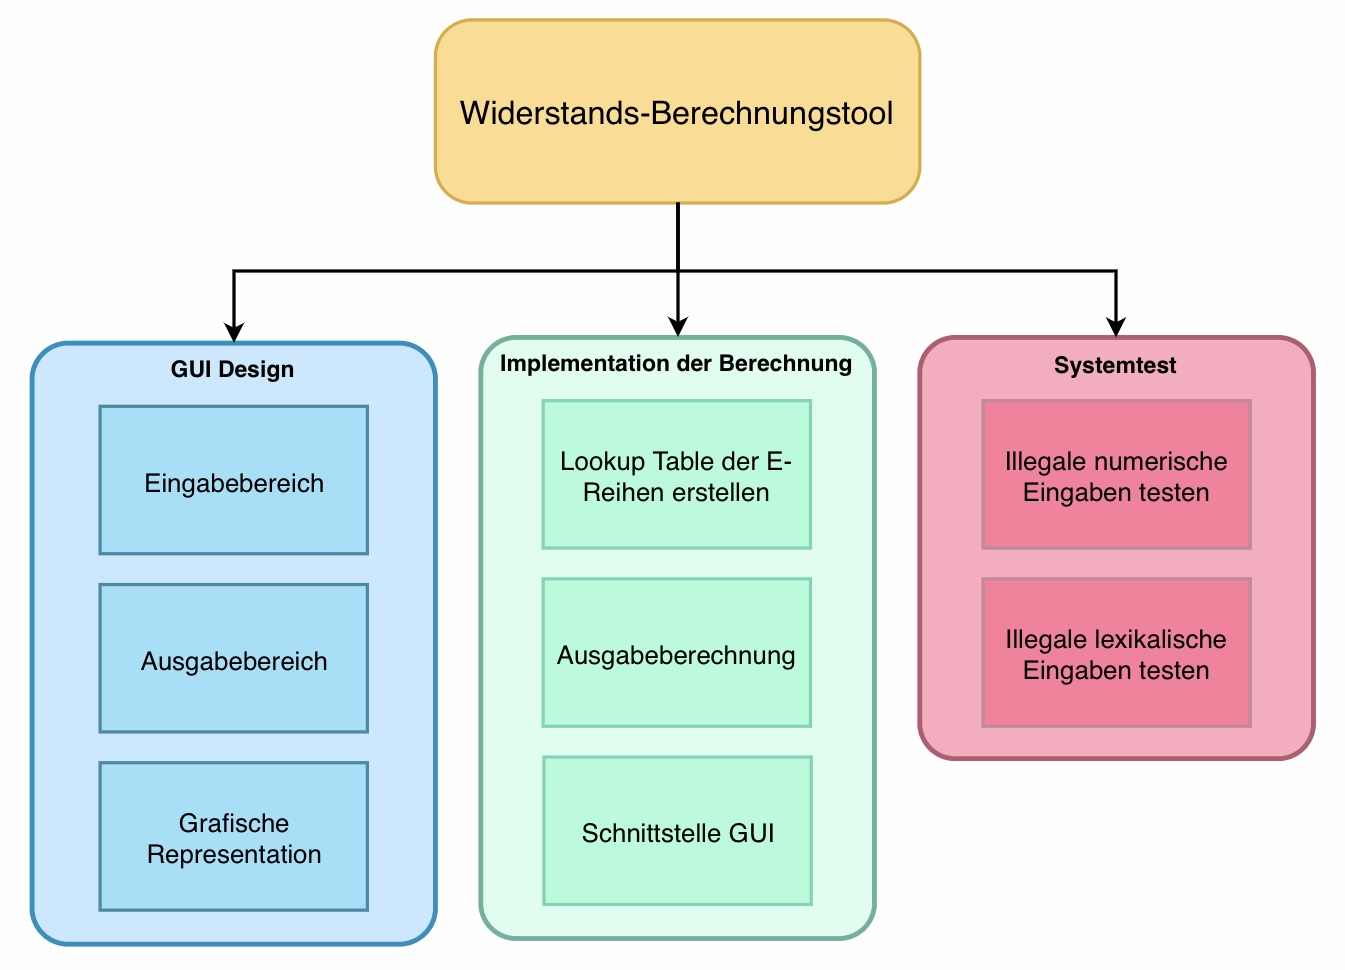
\includegraphics[width=14cm]{images/Projektstrukturplan}

\subsection{GUI-Design}
\subsubsection{Eingabebereich}
Design des Eingabebereiches mit Textboxen, Beschriftungen, Einheiten sowie Auswahl der E-Reihe.
\subsubsection{Ausgabebereich}
Design des Ausgabebereiches mit Lables, sowie Einheiten.
\subsubsection{Grafische Representation}
Schaltungsschema grafisch darstellen.
\subsection{Implementation der Berechnung}
\subsubsection{E-Reihen}
Lookup Table der E-Reihen erstellen
\subsubsection{Ausgabeberechnung}
Berechnung der Widerstandswerte und Auswahl aus der E-Reihe.
\subsubsection{Schnittstelle GUI}
Designblöcke in Code einbinden.
\subsection{Systemtest}
\subsubsection{Illegale numerische Eingaben testen}
Abfangen von negativen Spannungen, sowie negativen Spannungsdifferenzen. 
\subsubsection{Illegale lexikalische Eingaben testen}
Abfangen von nicht-numerischen Zeichen, sowie Eingabe von "," statt ".".
